\chapter{Implementation}\label{ch:implementation}

\section{Preparation}\label{sec:preparation2}

\subsection{Selecting a blockchain network}\label{subsec:selection-of-blockchain-network}

As seen in \cref{tab:selection-of-blockchain-network}, the findings in~\cref{sec:voting-systems} can be applied as selection criteria for relevant \gls{Blockchain} networks (see \cref{subsec:comparison-of-turing-complete-blockchains}).
However, some properties mentioned in~\cref{sec:voting-systems} depend entirely on decisions relating to frontend design and code governance rather than the selected \gls{Blockchain}, e.g., whether the software is open-source.
These are displayed in gray in~\cref{tab:selection-of-blockchain-network}.

\begin{table}[H]
    \begin{tabularx}{\textwidth}{bCCCC}
        \hline
        \textbf{Property} & \textbf{Ethereum} & \textbf{Hyperledger Fabric} & \textbf{Polygon} & \textbf{Solana} \\
        \hline
        Auditability & \dblcmark & \dblcmark & \dblcmark & \dblcmark \\
        \hline
        Anonymity & \dblcmark & \cmark & \dblcmark & \cmark  \\
        \hline
        \rowcolor{lightgray}
        Usability & - & - & - & -  \\
        \hline
        \rowcolor{lightgray}
        Accessibility & - & - & - & - \\
        \hline
        Security & \dblcmark & \cmark & \dblcmark & \cmark   \\
        \hline
        Scalability & \xmark & \cmark & \cmark & \cmark  \\
        \hline
        \rowcolor{lightgray}
        Transparency & - & - & - & - \\
        \hline
        Incoercibility & \xmark & \xmark & \xmark & \xmark  \\
        \hline
    \end{tabularx}
    \caption{Comparison of blockchains based on voting system requirements}
    \label{tab:selection-of-blockchain-network}
\end{table}

All four \gls{Blockchain} networks possess most of the necessary properties.
Nevertheless, as shown in \cref{subsec:comparison-of-turing-complete-blockchains}, scalability is a major issue underlying \gls{Blockchain} technology in general.
For instance, even though the Ethereum Foundation is looking to improve Ethereum's protocol further, theoretically enabling it to process up to 100,000 \gls{TPS} in the future, as of the time of this writing, it cannot process enough transactions to facilitate national elections.
Conversely, other \glspl{Blockchain} compromise on similarly essential features to achieve a higher number of \gls{TPS}, e.g., security or network stability, the latter being an equally important scalability aspect.
Therefore, based on our evaluation of the available options (see \cref{subsec:selection-of-blockchain-network}) and after confirming those findings with an industry expert, we come to the conclusion that Polygon provides the optimal trade-off between security and scalability, leading us to select it as our preferred blockchain network for this project.

\subsection{Selecting the technology stack}\label{subsec:selection-of-tech-stack}

Many frameworks could be used to develop the server- and client-side of a decentralized electronic voting system.
However, we rely on a full Node.js integration due to its non-blocking \gls{IO} to ensure high scalability (see~\cref{subsec:node.js}).
Similarly, given the scalability advantages of monorepos (see~\cref{subsec:nx}), we utilize nx to manage the project's repository.
Additionally, keeping transparency in mind (see~\cref{sec:voting-systems}), an open-source project built with nx is more accessible to other developers as a resource for future research.

We use Next.js as a framework on the client side as it allows for server-side rendering, increasing the application's overall security (see~\cref{subsec:next.js}) and making it \glstext{SEO}-friendly.
Alternatively, we could have chosen to develop the client-side with Nuxt.js, which mimics most of Next.js's server-side and static rendering methods, while using Vue.js instead of React.js.
Nevertheless, Nuxt.js has a smaller community, arguably making React.js the preferable choice.

Although Next.js comes with its own routing framework for API calls, it is reasonable to use a separate framework for requests that handle database and \gls{SmartContract} actions.
Therefore, we utilize Nest.js, which eases the process of following best practices regarding the development of backend applications.
As illustrated in~\cref{subsec:nest.js}, Nest.js is specifically designed with scalability in mind;
moreover, it ensures high readability for developers with either an \gls{OOP} or \gls{FP} background.
Likewise, we handle  database-related aspects of the application using a PostgreSQL database since a broad spectrum of developers should be familiar with a \gls{ORDBMS} and PostgreSQL in particular (see~\cref{subsec:postgresql}).

\section{Setting up the workspace}\label{sec:setting-up-the-workspace}

\subsection{Creating a GitHub repository}\label{subsec:creating-a-git-repository}

\begin{figure}[h]
    \centering
    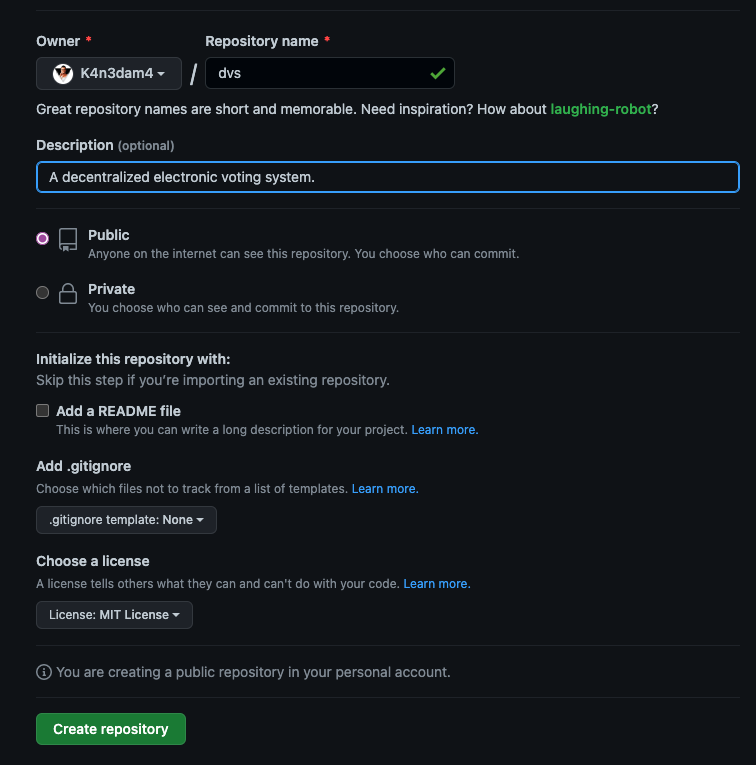
\includegraphics[scale=0.4]{boehm-initializing-repository}
    \caption[Creating a Github repository]{Creating a Github repository. Screenshot taken by author}
    \label{fig:initializing-repository}
\end{figure}

For the reasons discussed in~\cref{subsec:versioning}, the first step in the development process is the creation of a GitHub repository.
As seen in~\cref{fig:initializing-repository}, we change the license from \emph{None} to \emph{MIT License} to make this project available to the scientific community as a resource for further research.
Next, the repository is initialized, containing neither a README nor a .gitignore file, as these are automatically created by nx (see~\cref{subsec:creating-a-monorepo-using-nx}).

\subsection{Creating a monorepo using nx}\label{subsec:creating-a-monorepo-using-nx}

Creating a monorepo with nx is a straightforward process using the nx-provided executable package \emph{create-nx-workspace} with \gls{npx}.

\begin{figure}[h]
    \begin{subfigure}[b]{\textwidth}
        \centering
        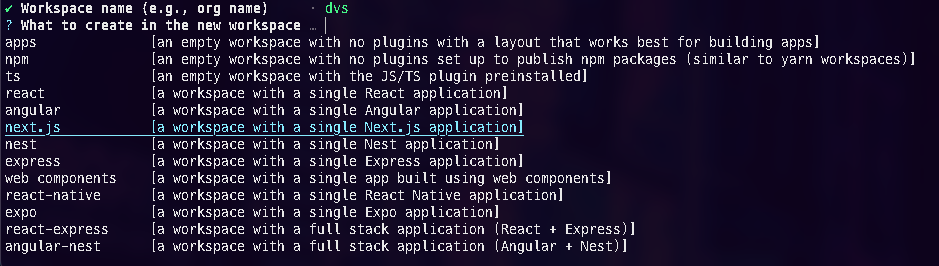
\includegraphics[width=\textwidth]{nx-workspace-options-0}
        \caption{Options for app templates nx can automatically build during initialization}
        \label{fig:nx-workspace-options-0}
    \end{subfigure}
    \begin{subfigure}[b]{0.5\textwidth}
        \centering
        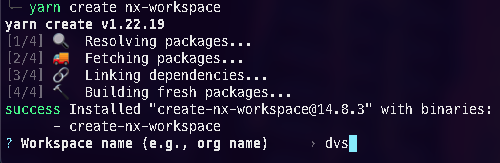
\includegraphics[width=\textwidth, height=85px]{nx-workspace-name}
        \caption{Naming the workspace}
        \label{fig:nx-workspace-name}
    \end{subfigure}
    \begin{subfigure}[b]{0.5\textwidth}
        \centering
        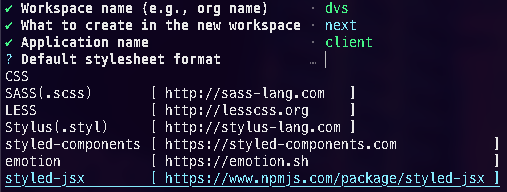
\includegraphics[width=\textwidth]{nx-workspace-options-1}
        \caption{Default style format options}
        \label{fig:nx-workspace-options-1}
    \end{subfigure}
    \caption[Setting up a nx workspace]{Setting up a nx workspace. Screenshots taken by author}
    \label{fig:setting-up-nx-workspace}
\end{figure}

After initiating the process by typing \mintinline[breaklines]{text}{yarn create nx-workspace} in the terminal, nx allows developers to name (see~\cref{fig:nx-workspace-name}) the project.
Next, developers are offered several template options for an initial application nx then automatically adds to the workspace (see~\cref{fig:nx-workspace-options-0,fig:nx-workspace-options-1}).
Given these options, we initialize the workspace with a Next.js application for the client side of the voting system.
Alternatively, we could initialize it containing a Nest.js application, but the order in which client and server applications are added to the workspace is irrelevant in this context.

\section{Setting up the backend}\label{sec:setting-up-a-nest.js-backend}

\subsection{Creating a Nest.js application}\label{subsec:creating-a-nest.js-application}

The installation of a plugin with \mintinline[breaklines]{text}{yarn add -D @nrwl/nest} is necessary to let nx handle the installation process of the Nest.js application.
After installing the plugin, we add a new Nest.js application to the workspace using the \mintinline[breaklines]{text}{nx g @nrwl/nest:app api} command, where \emph{server} is the name given to the application.

To maintain scalability, we combine Nest.js's modular design with nx's \emph{libs} directories, meaning backend controllers and services are kept as separate modules in \emph{libs/api} rather than the \emph{apps/server} directory.
As mentioned in~\cref{subsec:nx}, modularizing code within the \emph{libs} directory makes it reusable in all workspace applications sharing the same scope.
Hence, all future applications that might be added to the project will also be able to access that code if needed, thus making it easier to adhere to \gls{DRY} principles.

\subsection{Creating a PostgreSQL database}\label{subsec:creating-a-postgresql-database}

We create a new Nest.js module, \emph{prisma}, in the \emph{libs/api} folder, to handle database entries.
Then, we install Prisma as a devDependency with \mintinline[breaklines]{text}{yarn add -D prisma}, which provides basic tooling for databases, such as creating type-safe schemas, a built-in migration system, and a \gls{GUI} to display and edit database entries.
Following installation, we create a docker-compose.yml, enabling the application to run dockerized PostgreSQL databases during development, test, and production builds (see listing~\ref{lst:docker-compose.yml}).

\codeFromFile{yaml}{code_snippets/docker-compose.yml}{Docker-compose.yml used in the prisma module}{Docker-compose.yml used in the prisma module}{lst:docker-compose.yml}

Having created a docker-compose file, along with the commands necessary to run the database in the prisma module’s project.json and the project’s package.json, we can add a core Nest.js module (see listing~\ref{lst:core-module}).
The core module makes configurations such as the database \gls{URL} available throughout the Nest.js application.
We then proceed with connecting our Nest.js application to the database through the prisma service (see listing~\ref{lst:prisma-service}) using the \gls{URL} from the core module.

\codeFromFile{ts}{code_snippets/nest-core-module.ts}{Core module}{Core module}{lst:core-module}
\codeFromFile{ts}{code_snippets/nest-prisma-service.ts}{Prisma service}{Prisma service}{lst:prisma-service}

\section{Preparing for smart contract development}\label{sec:preparing-for-smart-contract-development}

\subsection{Setting up our IDE}\label{subsec:setting-up-our-ide}

Since our local \gls{IDE} (IntelliJ IDEA) does not natively support Solidity, our first step is to install the \emph{IntelliJ Solidity} plugin.
After installing the plugin, the \gls{IDE} should be able to recognize Solidity files (.sol) and provide us with basic syntax highlighting.
Unfortunately, the plugin does not provide autocomplete, making for an unpleasant development experience.

It should be noted that this is a problem specific to our preferred \gls{IDE}.
Developers running another \glsfirst{IDE}, such as VSCode or Atom, should be better equipped to write their Solidity code locally.
Nevertheless, since we do neither wish to switch to VSCode nor Atom, we will use the Remix \gls{IDE} to develop our \gls{SmartContract} online.

\subsection{Setting up Remix}\label{subsec:setting-up-remix}

As mentioned in \cref{subsec:remix-ide}, Remix Project provides us with an \glsfirst{IDE} and tools to deploy and debug our written code.
Although, we will later copy the code to our local workspace (see~\cref{subsec:setting-up-local-hardhat-project}) to use the contract's \gls{ABI} in the rest of our project.

\begin{figure}[h]
    \centering
    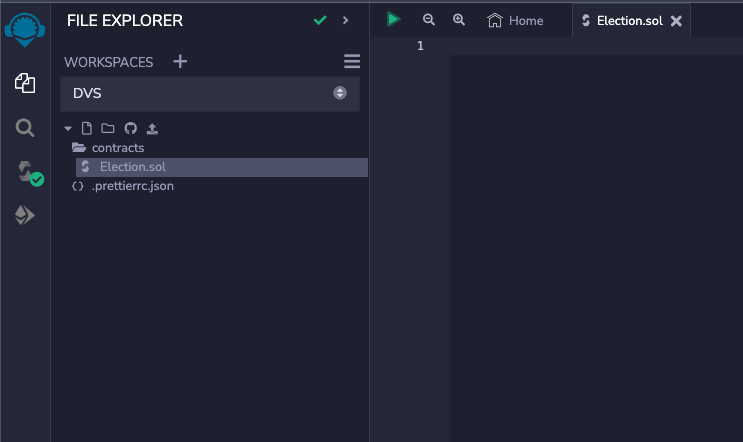
\includegraphics[width=\textwidth]{boehm-remix-startup}
    \caption[Setting up Remix]{Setting up Remix. Screenshot taken by author}
    \label{fig:remix-setup}
\end{figure}

Opening Remix \gls{IDE} for the first time, we see several example files in the \emph{contracts} and the \emph{scripts} directory.
So after deleting those, we create a new file in the \emph{contracts} folder called \emph{Election.sol} (see~\cref{fig:remix-setup}).

\subsection{Setting up local Hardhat project}\label{subsec:setting-up-local-hardhat-project}

Since our backend will depend on the \gls{ABI} of our written contract, we still need to set up a local project.
First, we use the nx command \mintinline[breaklines]{text}{nx g lib smart-contracts} to create a new nx library.
Afterward, we need to install the necessary Hardhat dependencies in our project's root directory

\begin{minted}[breaklines]{shell-session}
    yarn add -D hardhat @nomicfoundation/hardhat-toolbox
\end{minted}

and chai matchers to enable local testing of our election contract, as well as typechain, since we are going to need typed interfaces of our contracts

\begin{minted}[breaklines]{shell-session}
    yarn add -D @nomicfoundation/hardhat-chai-matchers @types/chai @types/mocha typechain @types/typechain @ethersproject/providers
\end{minted}

After installing all necessary dependencies, we configure Hardhat and tell it to run within its own directory in \emph{libs/smart-contracts} by creating a \emph{hardhat.config.ts} (see listing~\ref{lst:hardhat-config}) and adding nx commands for testing and compilation to the library's \emph{project.json} (see listing~\ref{lst:hardhat-project.json}).

\codeFromFile{ts}{code_snippets/hardhat-config.ts}{Hardhat config}{Hardhat config}{lst:hardhat-config}
\codeFromFile{json}{code_snippets/hardhat-project.json}{Hardhat project.json}{Hardhat project.json}{lst:hardhat-project.json}

\section{Smart contract}\label{sec:smart-contract}

To begin writing the \gls{SmartContract}, we will later deploy when \glsplural{Admin} create an election; we switch to Remix \gls{IDE} and open the \emph{Election.sol} file we created earlier.

\subsection{Selecting a Solidity compiler and language version}\label{subsec:selecting-a-solidity-compiler-and-language-version}

In contrast to code written in JavaScript, Solidity compiles to bytecode.
Hence, we need to start every .sol file we create with a \emph{compiler directive}, known as \emph{version pragma}~\autocite[135]{antonopoulos_mastering_2019}, that specifies the compiler and language version our contract expects

\begin{minted}[breaklines]{solidity}
// SPDX-License-Identifier: MIT
pragma solidity ^0.8.17;
\end{minted}

Our contract will be using Solidity 0.8.17, as well as higher minor versions, e.g., 0.8.20.

\subsection{Importing Ownable.sol}\label{subsec:impotring-ownable.sol}

Since some functions in the contract will only accept transactions from the \gls{Admin} address that created the election, we also import \emph{@openzeppelin/contracts/access/Ownable.sol} into our contract's context

\begin{minted}[breaklines]{solidity}
// SPDX-License-Identifier: MIT
pragma solidity ^0.8.17;
import "@openzeppelin/contracts/access/Ownable.sol";
\end{minted}

The OpenZeppelin library is a collection of reusable \glsplural{SmartContract} that include operations commonly needed when developing \glsplural{SmartContract}.
In this case, \emph{Ownable.sol} provides a basic ownership model for our contract, including functions for checking its current owner and transferring ownership to other \glsplural{Admin}.

\subsection{Defining the contract's structs}\label{subsec:defining-the-contracts-structs}

Since the data pertaining to an election can be split up into information about its candidates, voters and result, we use the struct data type to define how this data will look (see listing~\ref{lst:election-step1.sol}).

\codeFromFile{sol}{code_snippets/election-step1.sol}{Defining the contract's structs}{Defining the contract's structs}{lst:election-step1.sol}

\subsection{Defining the contract's states, constructor and modifiers}\label{subsec:defining-the-contract's-states-constructor-and-modifiers}

\codeFromFile{sol}{code_snippets/election-step2.sol}{Defining the contract's states, constructor and modifiers}{Defining the contract's states, constructor and modifiers}{lst:election-step2.sol}

\subsubsection{States}

Subsequently, as shown in listing~\ref{lst:election-step2.sol}, we use these data structures to define the contract's states: 

\begin{enumerate}
    \item The election's name
    \item The expiration timestamp
    \item A mapping of all registered voters, which acts as a hash lookup table iterable with a voter's wallet address~\autocite[137]{antonopoulos_mastering_2019}
    \item An array of the election's candidates
    \item An array of the result
\end{enumerate}

In elections conducted on the \gls{Blockchain}, having a dedicated state holding the election's expiration is essential.
Again, as discussed in~\cref{subsec:blocks}, once a transaction has been saved on the \gls{Blockchain}, it cannot be deleted.
Thus, the only possible way to prevent people from voting once an election has expired or an election official has closed it, is to change one of the contract's states to a value that will be checked by its functions before executing them.

\subsubsection{Constructor}

As in other programming languages, a contract's constructor is called only once when a new contract instance is created on the \gls{Blockchain}.
At first, we did not write arguments for the constructor since we assumed we would only deploy a single contract that could handle the creation of multiple elections by \glsplural{Admin} through the contract's \gls{ABI}.
However, we discussed this with an industry expert during our iterative process and were advised to rethink our concept as contracts can only hold a limited amount of data.
Moreover, designing a contract that manages multiple elections would be more challenging due to Solidity's limitations regarding data structures.
As a result, the final contract constructor accepts three arguments, the election's name, its candidates and expiration timestamp, which will be parsed to the contract during deployment (see listing~\ref{lst:election-step2.sol}).

\subsubsection{Modifiers}

The last thing we do before writing the contract's functions is to create a modifier that checks the value saved in the \emph{expires} state against the global variable \emph{block.timestamp}, which is exposed by the \gls{EVM}.
Since every transaction, including transactions that would change the contracts states, have to be added to a block, and each block has a timestamp, we can prevent successful state changes by adding the \emph{checkExpired} modifier to selected functions.

\subsection{Contract functions}\label{subsec:contract-functions}

The \gls{Admin} wallet address will primarily perform transactions on our contract through our Nest.js backend.

\codeFromFile{sol}{code_snippets/election-step3.sol}{Contract functions}{Contract functions}{lst:election-step3.sol}

\subsubsection{registerVoter}

As shown in listing~\ref{lst:election-step3.sol}, this function is only executable by the contract owner while the election has not expired.
It takes a voter’s wallet address as an argument, which will be created in our Nest.js backend when a voter tries to register for an election (see~\cref{subsec:admin-service}), and adds it to the voters mapping.
Lastly, it transfers a small number of funds from the \gls{Admin} wallet to the voter’s wallet to enable the latter to pay for transactions while interacting with the \gls{SmartContract}.
We also considered fully decentralizing the registration process.
However, we concluded that voters could not be expected to create their wallets as this remains unintuitive (see~\cref{subsec:election-service}).

\subsubsection{addVotingWeight}

This function (see listing~\ref{lst:election-step3.sol}) enables \glsplural{Admin} to add voting weight to a registered voter.
When a voter has no voting weight left, he is not eligible to vote.
This function may seem unnecessary in elections where voters only have one vote, but it could be used in later versions of the systems to create more complex elections.

\subsubsection{vote}

A voter sends a transaction calling the contract's vote function by using a private key related to a registered address (see~\cref{subsec:asymmetric-key-cryptography,subsec:elliptic-curve-cryptography}).
The function then subtracts voting weight from the voter and adds one vote to the candidate specified in its parameter (see listing~\ref{lst:election-step3.sol}).

\subsubsection{closeElection}

\Glsplural{Admin} can close elections by calling this function.
As seen in listing~\ref{lst:election-step3.sol}, the function sets the election's \emph{expires} state to the current block timestamp, preventing further transactions and calculates the election's result.

\subsection{Testing the contract}\label{subsec:testing-the-contract}

After successfully debugging and testing our contract on Remix, we copy it to our local \emph{libs/smart-contracts/src/lib/contracts} directory and try to compile it by running \mintinline[breaklines]{text}{nx compile smart-contracts} in our terminal.
Having installed \emph{typechain} earlier, this should create a new \emph{typechain-types} folder containing typed interfaces of our contract and its \gls{ABI}.

We now have everything we need to create a new \emph{test} directory and write tests for the contract (see listing~\ref{lst:election-tests.ts}).
Running unit tests on the contract provides valuable information about its functionality.
For example, initially, we checked the provided expiration timestamp in milliseconds against the global Solidity variable \emph{block.timestamp}, which is saved in seconds.
As the expiration time is a core element of elections, we fix this by multiplying the block timestamp by 1000 before comparing it to the expiration state.

\codeFromFile{ts}{../libs/smart-contracts/src/lib/test/Election.ts}{Testing the contract}{Testing the contract}{lst:election-tests.ts}

\section{Verifying the contract}\label{sec:verifying-the-contract}

We need to verify the \gls{SmartContract} to make elections fully transparent (\cref{subsec:qualitative-objectives,sec:voting-systems}).
This will later enable anyone who wishes to audit an election to visit a \gls{BlockExplorer} and execute all non-administrative contract functions in a web interface.

We prepare the project to handle contract verifications through the use of \gls{CLI} commands by adding

\begin{minted}[breaklines]{ts}
  etherscan: {
    apiKey: {
      polygonMumbai: process.env.POLYGON_SCAN_API_KEY as string,
    },
\end{minted}

to the \emph{libs/smart-contracts/hardhat.config} file.
We then add a new run target to the library's \emph{project.json} and set its command key to \mintinline[breaklines]{text}{npx hardhat verify 0x{args.address} --constructor-args {args.constructor_args} --network testnet}.
Subsequently, we are be able to verify a contract after its deployment by running the target from the project's root with the required arguments.
It should be noted, that \glsplural{BlockExplorer} compare the bytecode of contracts in newly mined blocks to the bytecode of all verified contracts.
No additional actions are required to make elections auditable when administrators create a new election using a contract version that has already been verified.

\section{Server}\label{sec:server}

Even though elections will exist as \glsplural{SmartContract} on our chosen \gls{Blockchain} network, we will still handle transactions in our Nest.js backend.

\subsection{Database}\label{subsec:database}

\codeFromFile{java}{../libs/prisma/prisma/schema.prisma}{Prisma schema}{Prisma schema}{lst:schema-prisma}

For this we install prisma into our project, create a prisma library and add a database schema (see listing~\ref{lst:schema-prisma}):

\begin{enumerate}
    \item Users
    \item Registered Voters
    \item Eligible Voters
    \item Elections
\end{enumerate}

After speaking with an industry expert, we decided to implement a single schema for users instead of an \gls{Admin} and a voter schema.
This enables us to handle all user requests with a single \gls{JWT} strategy using role guards (see \cref{subsec:security}).

\subsection{Core module}\label{subsec:core-module}

\subsubsection{Configuration}

As seen in listing~\ref{lst:core-config}, to enable certain features within our backend services, we first need to add a configuration file to the application's core which then parses information from our \emph{env} files to their relative configuration keys.

\codeFromFile{java}{../libs/api/src/lib/core/configuration.ts}{Core configuration}{Core configuration}{lst:core-config}

We use Alchemy as a provider for transactions on the \gls{Blockchain}, hence we need to add an Alchemy \gls{API} key to our env, which our configuration file processes.

\subsubsection{Ethers for Nest.js}

As our backend services will handle contract transactions, we first install nestjs-ethers in our project by typing \mintinline[breaklines]{text}{yarn add nestjs-ethers} in our terminal.
Ethers is a JavaScript library that provides several functions and methods to set up a provider quickly, deploy elections using our contract \gls{ABI}, and make transactions.

Next, we set up a new ethers module in the application's core by adding it to the import array and specifying the provider we want to use and the \gls{Blockchain} network on which we wish to deploy our contracts.
In our case, we use Alchemy and deploy contracts to Polygon’s Mumbai test network (see listing~\ref{lst:ethers-in-core}).

\codeFromFile{ts}{code_snippets/ethers-in-core.ts}{Ethers core module}{Ethers core module}{lst:ethers-in-core}

\subsection{Security}\label{subsec:security}

To prevent unauthorized entities from accessing protected pages (see~\ref{subsec:middleware}) or making requests to \gls{API} endpoints, we need to implement authorization services using \glsplural{JWT}.
We initially considered dispensing with user accounts since voter registration will be specific to an election.
However, we ultimately decided to implementing accounts to limit requests made to our server.

Hence, we first run \mintinline[breaklines]{text}{yarn add passport-jwt} in our terminal.
Then, we create three new files in \emph{libs/api/src/lib/guards} and \emph{libs/api/src/lib/strategies}, respectively.

As seen in listing~\ref{lst:jwt.guard.ts}, the \gls{JWT} guard intercepts each request to a route that injected with this guard and checks whether our \gls{JWT} strategy (see listing~\ref{lst:jwt.strategy.ts}) could validate the token in the request header.

\codeFromFile{ts}{../libs/api/src/lib/guards/jwt.guard.ts}{JWT guard}{JWT guard}{lst:jwt.guard.ts}
\codeFromFile{ts}{../libs/api/src/lib/strategies/jwt.strategy.ts}{JWT strategy}{JWT strategy}{lst:jwt.strategy.ts}

In order to protect \gls{Admin} routes, we employ user roles and inject the guard shown in listing~\ref{lst:role.guard.ts} as needed in our controllers.
Lastly, we create a \gls{JWT} module that can be imported into our main app module in \emph{apps/server/src/app} (see listing~\ref{lst:jwt.module.ts}).

\codeFromFile{ts}{../libs/api/src/lib/jwt/jwt.module.ts}{JWT module}{JWT module}{lst:jwt.module.ts}
\codeFromFile{ts}{../libs/api/src/lib/guards/roles.guard.ts}{Roles guard}{Roles guard}{lst:role.guard.ts}

Additionally, depending on the number of public routes in the application, it can make sense to guard all of them by default and then use Nest's \mintinline[breaklines]{ts}{Public()} decorator to selectively make certain routes public.
As our application will only have a public landing page and public \gls{API} endpoints for authorization and registration requests, we opt to protect all routes, open the core module and enable \gls{JWT} guards globally by adding them to the module's providers.

\begin{minted}[breaklines]{ts}
   providers: [
    {
      provide: APP_GUARD,
      useClass: JwtGuard,
    },
  ],
\end{minted}

\subsection{Admin service}\label{subsec:admin-service}

Since we decided to implement a \gls{GUI} to enable election officials to create new elections without prior experience in \gls{SmartContract} programming, we create methods to handle the creation and deployment in our server application.

As seen in listing~\ref{lst:create-election.ts}, the createElection service method first fetches the \gls{Admin}'s account.
Then we use nestjs-ether's EthersModule to create a signer with the \gls{Admin} \gls{PK} that is parsed from an .env to the server's configuration during the build process (see~\cref{subsec:configuration}) and create a local contract instance using the election contract \gls{ABI} and bytecode (see~\cref{subsec:setting-up-local-hardhat-project,subsec:configuration}).
The resulting factory has already been injected with the provider we specified in our core module (see~\cref{subsec:core-module}) and is ready for deployment in lines 11-15.
Finally, after the contract has been deployed successfully, we create a copy of the election in our prisma database.

\codeFromFile{ts}{code_snippets/create-election.ts}{Create election service}{Create election service}{lst:create-election.ts}

\subsection{Election service}\label{subsec:election-service}

Similarly to our considerations concerning the creation of elections, we concluded that voters could not be expected to create their own wallets.
Hence, we enable them to create and register a voter wallet through our election service.

For this, we configure the service to accept the voter's \gls{SSN}, which we then compare to a list of all \glsplural{SSN} in our database that are eligible to vote in the election (see listing~\ref{lst:register-voter.ts}).
Suppose the \gls{SSN} entered by the voter matches the hashed \gls{SSN} in his account and is listed among the eligible \glsplural{SSN} for this election.
In that case, we create a signer from a newly created wallet and instantiate the election's contract interface.
Next, we calculate current transaction fees on the \gls{Blockchain} network and use the election contracts' registerVoter function to register the voter's wallet address in the contract.
As shown in~\cref{subsec:contract-functions}, this will also transfer the funds specified in the function's parameter from the \gls{Admin} wallet to the voter wallet.
Subsequently, we add voting weight to the now registered voter, update our database entries, and return the voter wallets \gls{PK} as a mnemonic passphrase.

Since the voter is registered in our database with a newly created wallet address while the wallet's \gls{PK} is never saved on the server side, he has complete autonomy over the distribution of his voting weight while remaining entirely anonymous.

\codeFromFile{ts}{code_snippets/register-voter.ts}{Register voter service}{Register voter service}{lst:register-voter.ts}

\subsection{End-to-End tests}\label{subsec:e2e-tests}

To test our backend services, we use the \emph{server-e2e} application, which should have been automatically created in the \emph{apps/} directory by nx when we created the \emph{server} application.

\subsubsection{Ganache}

Since running \gls{E2E} tests of our backend services require transactions on a \gls{Blockchain} network, we install Ganache to run a local test network by typing \mintinline[breaklines]{text}{yarn add -D ganache} in our terminal.

\subsubsection{Tests}

\codeFromFile{ts}{code_snippets/e2e-test.ts}{Excerpt from server E2E tests}{Excerpt from server E2E tests. Tests requests from voters}{lst:server-e2e-tests}

As seen in listing~\ref{lst:server-e2e-tests}, aside from testing whether our services work as expected, we also test whether successful requests to controllers can only be made with the specified access rights and when request bodies contain expected data.

\subsubsection{Running the tests}

After writing \gls{E2E} tests for all backend services we can run our tests by using the following commands


\begin{minted}[linenos,breaklines]{shell-session}
    dotenv -e .env.test cross-var -- yarn ganache --account='0x%ADMIN_PK%,100000000000000000000' --account='0x%VOTER_PK%,0' & dotenv -e .env.test -- nx restart-db-test prisma && dotenv -e .env.test -- nx e2e server-e2e
\end{minted}

This starts a local \gls{Blockchain} network and creates an \gls{Admin} as well as a voter wallet.
After successfully starting the network, a clean test database will be started using our prisma module.
Lastly, our \gls{E2E} application will run the tests.

A comprehensive summary of the tests is available in~\cref{ch:apx-server-e2e-tests}, and the results will be analyzed and discussed in section~\cref{subsec:res-end-to-end-tests}.

\subsection{Scalability tests}\label{subsec:scalability-tests}

In order to evaluate the system's scalability, we create a Node.js application using nx.
This application generates a simulated list of voters and performs the \gls{E2E} voting process for each individual, either concurrently or consecutively.
By configuring a representative number of simulated voters, this test provides important insights into the system's operational costs and transaction speeds.

A comprehensive summary of the tests is available in~\cref{ch:apx-server-scalability-tests}, and the results will be analyzed and discussed in section~\cref{subsec:res-scalability-test}.

\section{Client}\label{sec:client}

As mentioned in~\cref{subsec:selection-of-tech-stack}, we utilize Next.js to develop the client side of our application.

\subsection{Configuration}\label{subsec:configuration}

As Next.js ships with its own tools for routing, including routing for \gls{API} requests, we first need to configure the application to reroute any traffic on \emph{/api} to the \gls{URL} of our backend server.
We can do this by creating a \emph{proxy.conf.js} file in the project's root directory (see listing~\ref{lst:proxy-conf.js}) and adding rewrites to the \emph{next.config.js} file (see listing~\ref{lst:next-conf.js}).

\codeFromFile{js}{../apps/client/proxy.conf.js}{Proxy configuration file}{Proxy configuration file}{lst:proxy-conf.js}
\codeFromFile{ts}{../apps/client/next.config.js}{Next configuration file}{Next configuration file}{lst:next-conf.js}

\subsection{Middleware}\label{subsec:middleware}

To protect our application's pages on the server side we use our backend's jwt services to check the user's jwt token on each request of a protected route.
We can achieve this by creating a \emph{middleware.ts} in the application's root directory (see listing~\ref{lst:next-middleware.ts}).

\codeFromFile{ts}{../apps/client/middleware.ts}{Next middleware}{Next middleware}{lst:next-middleware.ts}

\subsection{Pages}\label{subsec:pages}

\codeFromFile{jsx}{../apps/client/pages/election/all/index.tsx}{Election page}{Election page}{lst:election-page}

The client application consists of six pages, including pages for \glsplural{Admin} (see~\cref{tab:all-pages-accessible-on-the-client-side}).
We use Next.js's internal routing system to create those pages by adding an \emph{index.tsx} file to the \emph{pages} directory for the landing page.
Next.js treats folders within this directory as routes, so we create \emph{index.tsx} files for each page shown in~\cref{tab:all-pages-accessible-on-the-client-side} in their respective folders according to the routes we want to achieve.

Since we are adhering to atomic design principles, a page only fetches data on the server side from our backend services and renders organisms that contain most of our client-side logic.
Consequently, all pages are structured similarly (see listing~\ref{lst:election-page}).

\begin{table}[h]
    \begin{tabularx}{\textwidth}{p{4cm}>{\centering\arraybackslash}p{4cm}X}
        \hline
        \textbf{Page} & \textbf{Protected (user=\cmark/admin=\dblcmark)} & \textbf{Description} \\
        \hline
        Landing page & \xmark & When users open the voting system, they are greeted by a landing page.
        They will be able to log in or register by using the form located on this page. \\
        \hline
        Election overview & \cmark & The page consists of a slider displaying all current elections in the system. \\
        \hline
        Election page & \cmark & This page displays a single election.
        Here, users can register to vote, submit their ballot, and check an election's results once it has closed. \\
        \hline
        \Gls{Admin} overview & \dblcmark & This page displays analytical information about the voting system and its users.  \\
        \hline
        \Gls{Admin} create panel & \dblcmark & \Glsplural{Admin} can create new elections using the form on this page. \\
        \hline
        \Gls{Admin} election list & \dblcmark & \Glsplural{Admin} are provided with an additional page to inspect elections in the system.
        They also can manually close an election listed on this page. \\
        \hline
    \end{tabularx}
    \caption{All pages accessible on the client side}
    \label{tab:all-pages-accessible-on-the-client-side}
\end{table}